\documentclass{ctexart}
\usepackage{enumerate}
\usepackage[colorlinks,linkcolor=blue]{hyperref}

\usepackage{ulem} 
\usepackage{caption}
\usepackage{graphicx, subfig}


\title{霓虹歌姬企画}
\author{南方科技大学日语社}
\begin{document}
\maketitle
\tableofcontents

\section{前言}
前几天日语社的同学们一起去会展中心的伊势海老这个店吃日料,本来想着要不然跟服务员光说日语吧,看看会发生什么事。但是到了店里却觉得店员应该还是不可能懂日语的,遂作罢。我觉得如果想要日语炸店的话,还是要去些人均1000以上的店。虽说店员们不会说日语,可是店里依然飘荡着日语歌。几首歌听下来,觉得还挺好听的,就是我对这些歌曲和歌手都没有什么了解。同学们指出这是某某有名的歌手唱的有名的歌,我才猛然发现我虽然平素也是主要听日本的歌曲,但是对于ACG之外的日本歌曲其实并没有太多的了解。之前社里一起看红白歌会,回忆起廖同学讲着讲那讲得头头是道,加上我有点歌荒,不禁觉得是时候扩展一下我的听歌范围了。之前的我连安室奈美惠都不知道,多亏廖同学指点才算是知道了这么个人名。听歌就像看论文一样,看得多了写个综述是很好的。综述这种东西既有利于自己总结,也便于跟别人分享。遂决定组织各位写这么一个小小的综述集子,来看看日本到底有多少值得注意的歌手。每个词条大概有一张图片,再配上编写者的一些说明,最后给新人一个听歌的顺序,使得新人可以循序渐进地了解与习惯这个歌手的风格。歌手按虚拟偶像,声优,ACG歌手和非ACG歌手分类,方便读者检索。\\
“霓虹歌姬企画”这个名字是我拍脑袋定的。之所以叫歌姬是因为觉得这样叫比较萌。总之就是这样一个集子,感谢各位的贡献。——张子健


\section{虚拟偶像}
\subsection{$\mu$'s}
\begin{figure}[h]
\centering
 
\includegraphics[width=1.0\textwidth]{lovelive.jpg}
 \caption{LoveLive!}
\end{figure}
$\mu$'s是LoveLive!企划里校园偶像组合的名字。“为了拯救濒临废校的学校,九位少女决定组成校园偶像”。我觉得校园偶像这个设定还是很好玩的。我刚入学的时候曾经想要为了\sout{跟妹子玩耍}宣传南科大,在学校里组织一个校园偶像团体。可是实在是找不到合适的妹子,遂作罢。\\
与同一类型的偶像大师相比,虽说LoveLive!的动画做得显然没有偶像大师765要好,但是歌还是很好听的。我个人认为LoveLive!的音乐更胜一筹。其音乐人藤泽庆昌也是少女歌剧和宝石之国的音乐人。\\
LoveLive!的乐趣还在于丰富的真人生放送节目。LoveLive!实际上是一个2.5次元企划,因为虚拟偶像背后的声优本身在企划中也有很多的亮相机会。尤其是当动画本身做得不好的时候,真人节目就变得尤为重要。各位还可以在听了一定量的歌曲之后去找$\mu$'s的演唱会看看。粉丝们的热情与小姐姐们卖力的表演可以感动任何一个有偶像之魂的人。(小姐姐一词据说就是先从LoveLive!的粉丝圈子里面流行起来的)
\subsubsection*{歌曲推荐}
实际上$\mu$'s的曲风还是比较多变的。在这里列出一些笔者喜欢的歌。其中soldier game每次去KTV都想唱...
\begin{enumerate}
\item Angelic Angel
\item No brand girls
\item soldier game
\item 春情ロマンティック
\item Music S.T.A.R.T!!
\end{enumerate}

\subsection{偶像大师 百万现场}
偶像大师是万代南梦宫

\section{专职歌手}
\subsection{Aimer}

\begin{figure}[h]
\centering
 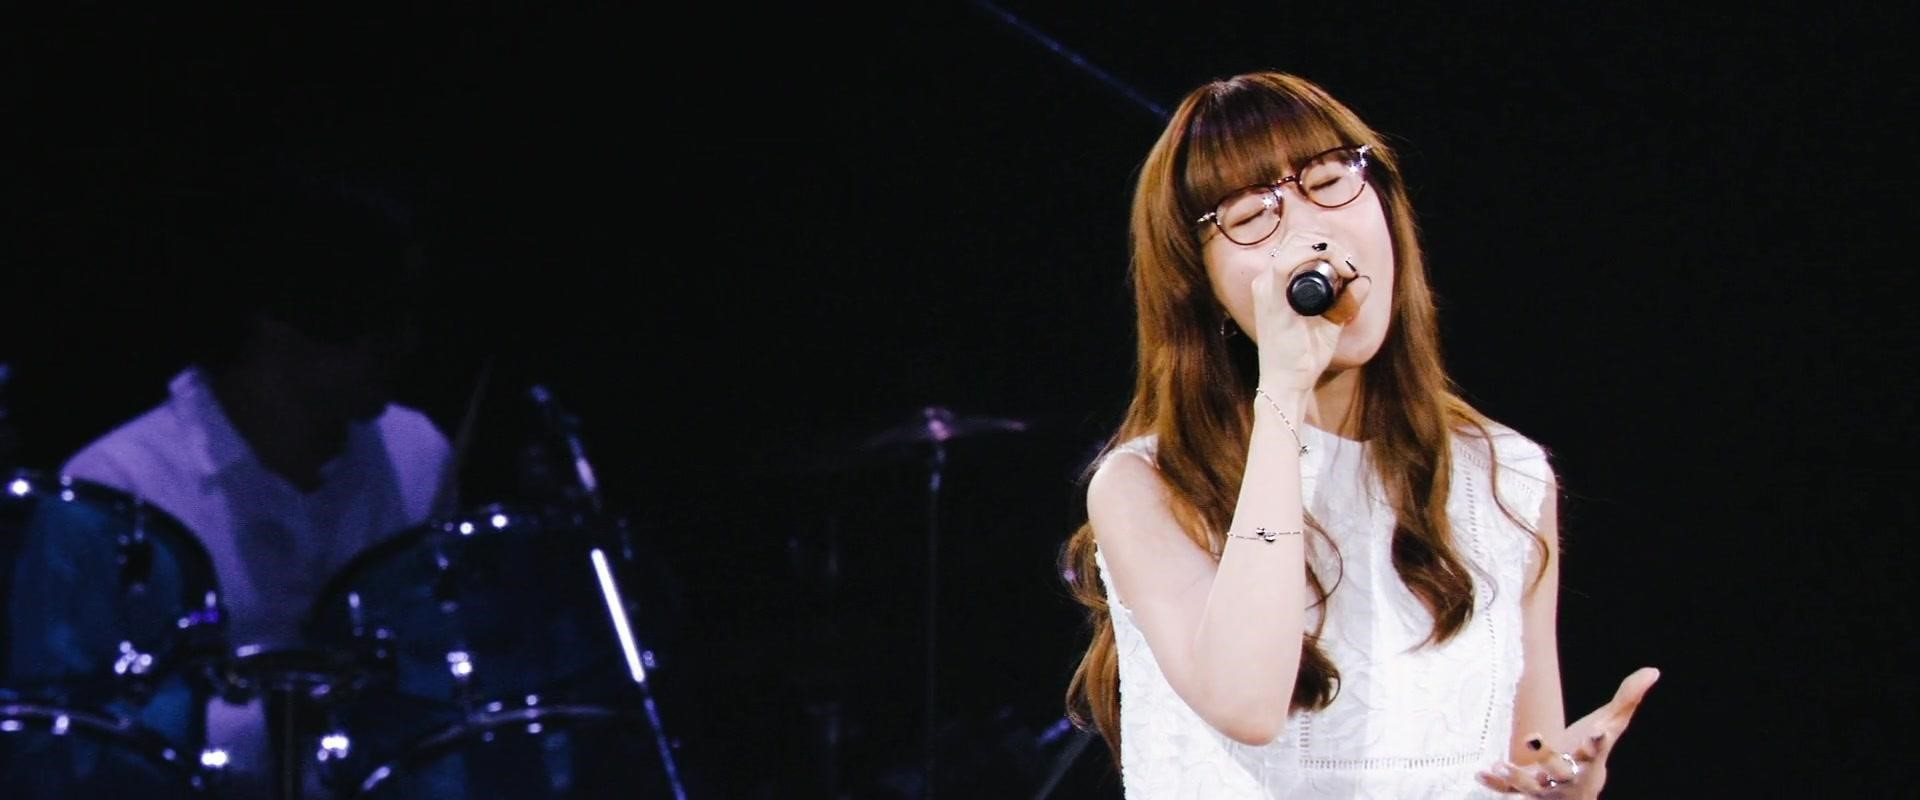
\includegraphics[width=1.0\textwidth]{Aimer.jpg}
 \caption{Aimer}
\end{figure}

想了很久,还是把Aimer放在了第一位。所谓第一位,其所指就是在笔者眼中,作为一位歌姬,Aimer的存在就其音乐上的魅力是无可比拟的。\\
Aimer15岁时喉部病变,一度难以说话。但因祸得福,随着嗓音的逐渐变化,Aimer开发出了一种极为独特的声线,一种令人难以自拔乐不思蜀抚掌击节余音绕梁的声线。孔子有“三月不识肉味”的赞美,我想也不过如此。\\
当然Aimer如今的成就离不开制作人agehasprings的提携。一单《六等星之夜》便一炮而红,她优雅而纯净,略有沧桑但返璞归真的嗓音俘获了大量粉丝。一单之后Aimer开始不断地为TV动画献唱,进一步累积人气。2017年8月29日,Aimer在武道馆进行了首次live,首次以戴眼镜的形象示于众人,令人眼前一亮。Aimer虽然也算是新人歌姬,但现场发挥却十分稳定,丝毫感受不出首次live的紧张感,极有表现力。\\
值得一提的是,今年4月,Aimer五专就会发售,收录了近两年的人气曲目,赶紧买买买。\\
然而就客观而言,Aimer的音乐成就还没有达到前辈们的高度,但随着人气的攀升,假以时日,笔者相信Aimer会成为又一代天后。\\

\subsubsection*{歌曲推荐}
Aimer的歌,基本都收录在“两只猫”里,名字叫BEST SELECTION “blanc” 与“noir”,买一张听一辈子。一张猫专就能满足对一天生活的所有期待。
\begin{enumerate}
\item 茜さす
\item あなたに出会わなければ
\item 花の唄
\item 悲しみはオーロラに
\end{enumerate}


\end{document}